% 编辑器使用说明
% 小时物理百科|在线编辑器|latex

\subsection{零基础视频教程}
\begin{enumerate}
\item 使用入门(\href{https://www.bilibili.com/video/av87698355/}{B 站}, \href{https://zhuanlan.zhihu.com/p/105869878}{知乎})
\item 提高编辑效率 (未完成)
\end{enumerate}

\subsection{简介}
\begin{figure}[ht]
\centering
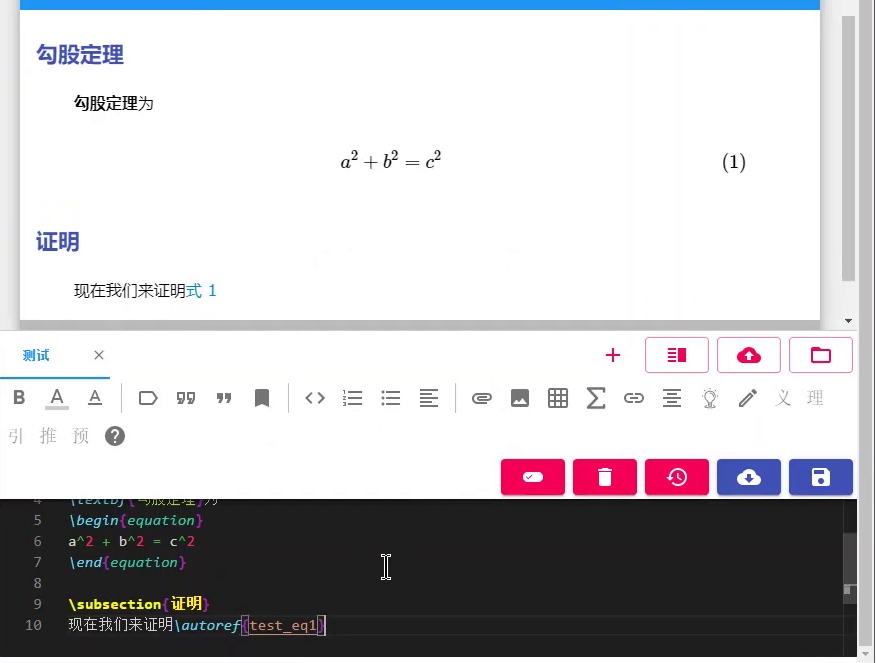
\includegraphics[width=10cm]{./figures/editor_3.png}
\caption{编辑器截图(\href{http://wuli.wiki/apps/editor.gif}{GIF 动画})} \label{editor_fig3}
\end{figure}

\begin{itemize}
\item 编辑器可从网站首页的链接进入(必须处于登录状态). 如果不想注册, 可以使用测试网址 \href{http://wuli.wiki/editor}{wuli.wiki/editor}, 测试账号为 \lstinline|test1| 到 \lstinline|test100|, 密码 6 个 8. 注意测试文件会被定期删除, 可以自行使用下载按钮备份
\item 目前该编辑器仅用于编辑百科词条, 我们正在开发个人笔记功能(\href{http://wuli.wiki/editor?target=home}{测试页面}), 让每个用户都可以创建自己的百科
\item 进入编辑器初始页面后, 点 “新建词条” 图标(红色加号)可以新建文件, 点 “打开词条” 图标可以编辑已有文件. 新建或修改的内容不会立即更新到网站, 而是要审核通过才会发布(有发布权限的用户可以自行发布). 可以在\href{http://wuli.wiki/changed/changed.html}{这里}查看新建或修改中的词条
\item 编辑过程中用快捷键 Ctrl+S 可以保存并刷新预览(建议经常刷新, 便于定位错误). 也可以用工具栏的保存图标.
\item 本编辑器使用 LaTeX 语言的一个子集, 一个简单的 LaTeX 介绍见 “LaTeX 简介\upref{latxIn}”
\item 注意这并不是一个通用的 LaTeX 编辑器, 只实现了一小部分命令. 工具栏有大部分常用命令, 所有命令见 “词条示例\upref{Sample}”
\item 新建或打开的每个词条文件并不是一个可独立编译的 .tex 文件而是一个 \lstinline|\section|, 详见下文
\item 我们在模板中用 \lstinline|\newcommand{}{}| 加入了一些自定义命令, 但不会覆盖原有的 LaTeX 命令.
\end{itemize}

\subsection{公式}
\begin{itemize}
\item 公式环境支持大部分 LaTeX 命令, 严格来说是所有 \href{https://www.mathjax.org/}{MathJax} 支持的命令\footnote{MathJax 项目用于在网页上显示 LaTeX 公式, \href{https://www.zhihu.com/}{知乎}的公式也使用 MathJax.}.
\item 一个简单的公式编辑器见\href{https://www.codecogs.com/latex/eqneditor.php}{这里} (不建议使用, 建议练习手动输入)
\item 一个简单的 TeX/LaTeX 公式入门教程见\href{https://chaoli.club/index.php/211}{超理论坛}
\item 支持部分 \href{http://mirrors.ibiblio.org/CTAN/macros/latex/contrib/physics/physics.pdf}{Physics 宏包}中的命令
\item 行内公式插入到两个美元符号之间, 如 \lstinline|$a^2+b^2=c^2$| 显示为 $a^2 + b^2 = c^2$.
\item 独立公式只能用 \lstinline|equation| 环境(推荐), \lstinline|align| 环境或者 \lstinline|gather| 环境. \lstinline|equation| 环境可以通过工具栏的公式图标插入, 也可以打 \lstinline|\beq| 然后按 Tab 键或者回车插入, 如
\begin{equation}\label{editor_eq1}
a^2 + b^2 = c^2
\end{equation}
\item 公式中所有常用的和自定义的命令见 “词条示例\upref{Sample}”
\item 为增加代码可读性, 编辑器中一些命令会显示为对应的符号(如希腊字母, 求和符号, 不等号等), 注意这不会影响源码(复制时得到的也是命令而不是符号). 以后会增加一个开关选择是否关闭该功能.
\item 工具栏中的 “内部引用” 按钮可以引用同一页面的公式并生成链接(图片表格等同理), 如\autoref{editor_eq1}. “外部引用” 按钮可以引用其他词条的公式或图表.
\end{itemize}

\subsection{用户权限}
每个注册用户默认有编辑词条的权限, 但却不能直接发布词条, 而是需要由发布权限的用户审核后发布. 若一个词条处于 “编辑中” 的状态, 则其他用户无法修改该词条, 只能以只读模式打开. 新建或修改的词条只有通过审核并被发布后才可以被其他用户重新编辑. 所有编辑中的词条页面都可以在\href{http://wuli.wiki/changed/changed.html}{临时页面}(\autoref{editor_fig1})查看. 括号中会显示修改该词条的用户.

\begin{figure}[ht]
\centering
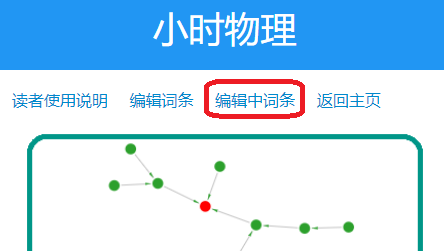
\includegraphics[width=9cm]{./figures/editor_1.png}
\caption{从 \href{http://wuli.wiki/online}{wuli.wiki/online} 查看编辑中的词条} \label{editor_fig1}
\end{figure}

\subsection{文件结构}

百科的所有词条是 LaTeX 的一个 \lstinline|document| 环境, 目录中每个 “部分” 是一个 \lstinline|\part|, 每个 “章” 是一个 \lstinline|\chapter|, 每个词条是一个 \lstinline|\section|, 词条中蓝色的小标题是 \lstinline|\subsubsection|, 黑色的小标题是 \lstinline|\subsubsection|. 编辑器打开的一个词条文件就是一个 section 的内容(不需要 \lstinline|\section| 命令). 用 TeXlive 编译 pdf 的时候所有词条文件都会通过 \lstinline|\input{xxx.tex}| 插入到主文件 PhysWiki.tex 中.

网页版的词条目录(\href{http://wuli.wiki/online/}{wuli.wiki/online/})由 PhysWiki.tex 文件生成, 所以必须修改该文件并发布才能更新目录.

每个词条文件(后缀名为 tex)都有一个独一无二的文件名, 可以将通过将光标停留在编辑器中的 tab 上查看.

\begin{figure}[ht]
\centering
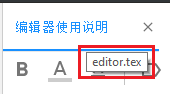
\includegraphics[width=4cm]{./figures/editor_2.png}
\caption{查看词条文件名} \label{editor_fig2}
\end{figure}

每个词条(section) 的 label 与文件名相同, 转换后输出的网页文件(html)也有相同的文件名, 可以在浏览器的地址栏中看到(例如本文的 LaTeX 文件是 \lstinline|editor.tex|, label 是 \lstinline|editor|, 转换成网页为 \lstinline|editor.html|).

\subsection{编辑器说明}
\begin{itemize}
\item 将光标停留在任意按钮上都会出现提示说明按钮的名称. 要新建词条, 点击红色的加号按钮, 根据提示新建即可. 要打开已有词条, 点击最右边的打开, 搜索需要的词条即可
\item 正文中请使用中文标点, 编辑器会自动把空心句号替换为全角实心句号
\item 编辑器会将有改动的词条每隔 5 分钟备份一次, 可以用 “恢复” 按钮恢复历史版本
\item 按下保存按钮(快捷键 \lstinline|Ctrl + S|) 会自动保存并编译
\item 编辑器支持各种自动引用(被引用对象没有 label 时会自动插入 label), 工具栏上的\textbf{内部引用}按钮可以引用同一词条的公式, 图表, 例题等环境. \textbf{外部引用}按钮可以引用其他词条的各种环境
\item 如果要在网页预览和 LaTex 代码之间跳转到对应位置, 可以通过搜索关键词实现. 例如在预览窗口复制一段文字, 在编辑窗口搜索就可以跳转到对应内容
\item 任何时候打出反斜杠会自动提示, 用 tab 键自动补全, 用上下键选择. 候选词未必是从最左边开始匹配, 例如打 \lstinline|\bf| 按 tab 就会得到 \lstinline|\textbf{}|
\item 如果自动补全带括号, 例如 \lstinline|\frac{}{}|, 补全后光标会自动进入第一个大括号, 再次按 tab 光标会跳到第二个括号, 再按 tab 光标会跳到第二个大括号外.
\item 打 \lstinline|\beg| 按 tab 会自动出现 \lstinline|\begin{}...\end{}|, 在 \lstinline|begin| 中输入环境名时, \lstinline|end| 中的环境名也会同步. 输完以后按 tab, 光标会跳到环境内
\item 打 \lstinline|\beq| 按 tab 会自动出现 \lstinline|\begin{equation}...\end{equation}|
\item 打 \lstinline|\bit| 按 tab 会自动出现 \lstinline|\begin{itemize}...\end{itemize}|
\end{itemize}


\subsubsection{快捷键}

\begin{table}[ht]
\centering
\caption{编辑器快捷键}\label{editor_tab1}
\begin{tabular}{|c|c|c|c|}
\hline
保存词条 & \lstinline|Ctrl + S| & 打开词条 & \lstinline|Ctrl + O| \\
\hline
新建词条 & \lstinline|Ctrl + Alt + N| & 关闭词条 & \lstinline|Ctrl + Alt + W| \\
\hline
显示编辑器选项 & \lstinline|Ctrl + Q| & 跳转到某行 & \lstinline|Ctrl + G| \\
\hline
查找文本 & \lstinline|Ctrl + F| & 替换文本 & \lstinline|Ctrl + H| \\
\hline
向左缩进 & \lstinline|Ctrl + [| & 向右缩进 & \lstinline|Ctrl + ]| \\
\hline
增大字号 & \lstinline|Shift + Alt + (+)| & 减小字号 & \lstinline|Shift + Alt + (-)| \\
\hline
关闭不保存 & \lstinline|Shift + 点关闭| &  &  \\
\hline
\end{tabular}
\end{table}
